
\chapter{Introduction and motivation}
\label{Introduction} 

%1. Establishing your research territory
%2. Constructing the research gap or niche
%3. Pointing out the gap/niche
%4. Stating your purpose. Aim statement or research question
%5. Highlighting benefits and mapping out the paper


%1. Statements about the field of research
%to provide the reader with a setting or
%context for the problem to be
%investigated and claimed its centrality
%or importance.
%2. More specific statements about
%the aspects of the problem already
%studied by other researchers, laying
%a foundation of information already
%known.
%3. Statements that indicate the need for
%more investigation, creating a gap or
%research niche for the present study
%to fill.
%4. Statements giving the purpose/
%objectives of the writer's study or
%outlining its main activity or findings.
%5. Optional statement(s) that provide a
%positive value or justification for
%carrying out the study.

%\section{RISC-V and Open-source processors}

\section{Motivation}


With the end of Dennard scaling and the recent slowdown of Moore's Law, achieving performance and energy efficiency improvements from scaling down the transistors is getting exponentially harder \cite{hennessyComputerArchitectureQuantitative2019}. This has led to a shift from general-purpose processor cores to \acrfull{dsa}. Companies need to specialize their processors to achieve higher performance and lower energy instead of using an available general-purpose processor \cite{mezgerSurveyRISCVArchitecture2022}. 


The growing demand for specialized processors has also led to a demand for an open and modular \textit{Instruction Set Architecture (ISA)}. The RISC-V ISA \cite{watermanRISCVInstructionSet2019,watermanRISCVInstructionSet2021}, originally developed at UC Berkeley in 2010 \cite{pattersonComputerOrganizationDesign2021}, has recently gained popularity in academia and industry because of its open-source nature, proven RISC-style, and modularity \cite{asanovicInstructionSetsShould2014}. The ISA consists of a base architecture with the possibility to add functionality through various standard or custom extensions\cite{watermanRISCVInstructionSet2019}. This flexibility is particularly useful for \acrshort{dsa}s, allowing designers to start with a minimal processor, extend it with only the required extensions, and possibly add custom implementation-specific instructions. Custom extensions enable compute-intensive tasks to be implemented in hardware and accessed through custom instructions. 

Being an open-source ISA, anyone can use and modify RISC-V without a licensing fee. This allows a low barrier to entry and collaboration between developers and researchers. The open nature of RISC-V open-source ISA has also led to an increasingly large ecosystem of open-source processors. One such example is the CV32E40S \cite{OpenhwgroupCv32e40s2024}, a processor core from the CORE-V family of processor cores from the OpenHW Group, a global organization of many companies working together to make open-source cores, tools, and software \cite{taylorAdvancedRISCVVerification2023}. The CV32E40S is a relatively small and efficient processor with a 4-stage pipeline. The core can be configured to support different RISC-V extensions and also adds the custom Xsecure extension, adding multiple security features \cite{openhwgroupIntroductionCOREVCV32E40S2023}. This processor will be used as an example throughout the report.




%Previously, processor development has been done by a small handful of companies, but with the growing need for specialized processors, the need for an open and modular ISA has increased. 

\subsection{Processor verification \& the need for a reference model}

Compared to trusted commercial solutions, the biggest barrier to adopting open-source processor IPs in a System-on-Chip (SoC) is the core's quality, particularly the verification effort invested in the core. Compared to open-source software, hardware typically has a much higher manufacturing cost, increasing the verification requirements \cite{kevinmcdermottOpenHWIndustrialGradeVerification2022}.
With RISC-V, where "anyone" can make a processor, the verification responsibility is now moved from a few specialized IP suppliers to every SoC developer. 

Therefore, a versatile and open verification environment is essential to RISC-V's continuing popularity and growth. Verification is a crucial aspect of processor development, consuming a significant portion of the overall development time. If every developer team were to build their verification environment from scratch, the adoption of RISC-V would likely stagnate.

Conventional manual testing with predetermined outcomes can be time-consuming and inadequate to validate a processor's complex behavior thoroughly. Instead, constrained random testing is often used to generate a wide range of test stimuli, covering many test cases. Variations of the "step-and-compare" methodology are widely used for processor verification \cite{taylorAdvancedRISCVVerification2023}. The diagram in \Cref{fig:testbench_block_diagram} shows an example of this, where the \textit{Device Under Test (DUT)} processor core, written in \acrfull{rtl} code, runs in parallel with a golden \gls{rm} written in a higher level language, all in a \acrfull{uvm} testbench environment. 

The two run in lock-step, executing the same test program, one instruction at a time. 
The processor state of the DUT and reference model is usually compared after each instruction has been \gls{retired}, which is when the execution of the instruction has been completed, and all the state changes to registers and memory associated with the instructions have been updated \cite{taylorAdvancedRISCVVerification2023}. 

At the retirement of each instruction, the core and reference model outputs its state changes, which are compared by a comparison module. If a mismatch between the two is detected, this can be instantly flagged, instead of having to run through the entire test program and compare the results afterward. 

Asynchronous events such as interrupts and debug requests are injected into the core and reference module through \acrshort{uvm} agents, independently of the test program.

In RISC-V, the state of the processor is stored in multiple types of registers. The 32 \acrfull{gpr} are visible to the programmer, used for normal program execution, and are read from and written to by the instructions \cite{watermanRISCVInstructionSet2019}. Additionally, the \acrfull{pc} is the register that holds the address of the current instruction \cite{watermanRISCVInstructionSet2019}. There is also a set of registers that are used to control and monitor the operation of the processor, called the \acrfull{csr}. \tmp{bakgrunn?}

\begin{figure}
    \centering
    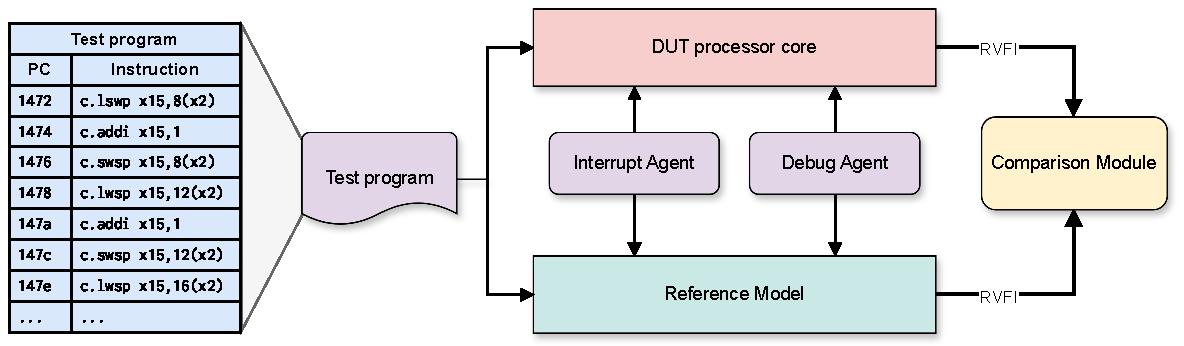
\includegraphics[width=0.75\linewidth]{figures/ISS_Testbench.pdf}
    \caption{Simple block diagram of a testbench with a reference model parallel to a processor core, running the same test program. }
    \label{fig:testbench_block_diagram}
\end{figure}




\subsection{The challenge of verifying asynchronous events}

For verification of normal instruction execution, using an \acrfull{iss}, simulating the processor at the instruction level granularity is often sufficient. However, the ISS becomes inadequate when \textit{Asynchronous events}, such as interrupts and debug requests, interrupting the normal program flow, are introduced \cite{taylorAdvancedRISCVVerification2023}. They pose a challenge because of the differing abstraction levels of the ISS and the RTL level of the DUT, which can lead to improper timing of interrupts and side effects. Asynchronous events in an ISS are synced to the beginning of an instruction, unlike in the RTL implementation, where asynchronous events can arrive at any cycle, and the timing can be affected by the state of the pipeline \cite{taylorAdvancedRISCVVerification2023}.

As a motivating example, that we will come back to later, consider the two instruction traces in \Cref{fig:lw_example}. This shows the instructions run by the core and ISS in a setup like \Cref{fig:testbench_block_diagram}, where we use an instruction-accurate ISS as the reference model. The figure shows that when they execute normal sequential code, they will both correctly run the same instructions. The problem arises when an interrupt is injected into both the core and ISS between PC 1524, and 1526. Since the ISS fully completes its execution of an instruction before moving on to the next, the interrupt handler starting at \rv{PC = 40}, is executed as the next instruction after the interrupt. In comparison, the core may have instructions in its pipeline that can not be interrupted, causing it to wait a few instructions before the interrupt is taken. 

Correctly predicting the delay between the interrupt injection and when the interrupt is taken, is one of the major problems with this verification strategy. The delay is highly dependent on core-specific functionality and cycle-accurate timing, making this delay hard to predict \cite{taylorAdvancedRISCVVerification2023}. 

The problem above becomes even more complicated when multiple different asynchronous events are triggered concurrently, as core-specific functionality affects how these events influence each other, which of them will be taken first, and how this affects the timing \cite{}. 

\begin{figure}
    \centering
    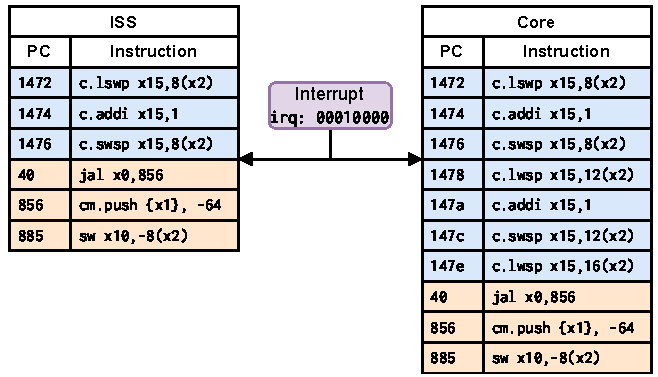
\includegraphics[width=0.75\linewidth]{figures/lw_add_sw_example.pdf}
    \caption{Simple example showing interrupt injection into an ISS and a core.}
    \label{fig:lw_example}
\end{figure}





%\begin{terminal}
%c.li x11,0
%c.addi x11,1
%c.addi x11,2
%c.addi x11,3
%c.addi x11,4
%c.addi x11,5
%
%c.lwsp x15,8(x2)
%c.addi x15,1
%c.swsp x15,8(x2)
%c.lwsp x15,12(x2)
%c.addi x15,1
%c.swsp x15,12(x2)
%c.lwsp x15,16(x2)
%\end{terminal}


%\section{Approach/scope of the report}

%
%


%\section{Requirements}
%\begin{itemize}
%    \item Cycle-level simulation
%    \item Run in async lock-step-compare with openHW core (e.g. CV32E40S)
%    \item Handle async events
%    \item handle hardware real-time effects
%    \item Pipeline understanding
%    
%\end{itemize}

\section{Objectives}

This report will focus on how a reference model can be built to properly simulate and verify asynchronous events by incorporating a pipeline understanding. 
%To overcome these limitations, the report will discuss the challenges in verifying asynchronous events and explore different approaches to building a reference model. The model will integrate a pipeline understanding and accurate interrupt simulation to solve these challenges.

\begin{enumerate}
    \item Highlight the complexities of verifying asynchronous events.
    \item Discuss the advantages and disadvantages of previous solutions.
    \item Design, architect, and implement a reference model to correctly simulate asynchronous events.
\end{enumerate}

\tmp{Hvilke spørsmål ønsker jeg å finne svar på og hva vil jeg løse gjennom arbeidet}

\section{Research Methodology}

\tmp{Hvilke typer aktiviteter er utført for å finne svar på spørsmålene i oppgaven?}

To achieve 

\section{Scope}

\begin{itemize}
    \item Implementation of CLINT interrupts, not CLIC, NMI, or debug requests, as many of the same principles apply to them. 
    \item Main focus on machine-level 
\end{itemize}

\section{Contributions}

\begin{itemize}
    \item Add Onespin support to core-v-verif
    \item Expand spike with enhanced rvfi support, injection of interrupts, state revertion, support for CV32E40S core
    \item Pipeline shell implementation
\end{itemize}


\section{Outline}

\begin{itemize}
    \item Introduction
    \item 
\end{itemize}

%\Cref{ch:Background} will describe how interrupts are handled in RISC-V and how they are affected by the pipeline. We will also describe common verification techniques and verification environments, and introduce different Instruction Set Simulators.
%
%\Cref{ch:Reference Model} will discuss the design and architecture of a reference model featuring a pipeline shell modeled around an existing ISS. We will compare different pipeline shell implementations, existing ISSs, and interfaces between the pipeline shell and the ISS. The CV32E40X core from the OpenHW Group will be used as an example processor to model. Still, we will also consider how the reference model can be easily configurable to different cores.
%

